% \PassOptionsToPackage{dvipdfmx}{graphicx}% only for Japanese
% \PassOptionsToPackage{dvipdfmx}{xcolor}% only for Japanese
\documentclass[sip,biber]{now-journal}
\addbibresource{IEEEabrv.bib}
\addbibresource{ref.bib}

\usepackage[nolist,nohyperlinks]{acronym}
\usepackage{amsfonts}
\usepackage{bm}
\usepackage{mathtools}
\usepackage{interval}
\usepackage{siunitx}
\usepackage[skip=1pt]{subcaption}

% reload hyperref
\usepackage[colorlinks=true, allcolors=blue, plainpages=false, pdfpagelabels=true]{hyperref}
\usepackage{breakurl}

% cleveref setting
\usepackage[capitalise]{cleveref}
\crefformat{equation}{(#2#1#3)}
\Crefformat{equation}{#2Equation~(#1)#3}
\crefformat{section}{Section~#2#1{}#3}
\crefname{algorithm}{Algorithm}{Algorithms}
\crefname{equation}{}{}
\crefname{figure}{Figure}{Figures}
\crefname{section}{Section}{Sections}
\captionsetup[subfigure]{subrefformat=simple,labelformat=simple}
\renewcommand\thesubfigure{(\alph{subfigure})}
\def\crefrangeconjunction{--}

% psuedo codes
\usepackage{xcolor}
\usepackage[theorems,skins]{tcolorbox}
\usepackage{tabularx}
\usepackage{pseudo}
\newtcbtheorem[crefname = {Algorithm}{algorithms}]{algorithm}{Algorithm}{pseudo/booktabs, float=t, theorem hanging indent=0pt}{alg}
\pseudodefinestyle{fullwidth}{
    begin-tabular=
    \tabularx{\textwidth}[t]{@{}
        r                                          % Labels
        >{\leavevmode\pseudosetup}                 % Indent, font, ...
        X                                          % Code (flexible)
        >{\leavevmode} % Comment styling
        p{0.20\textwidth}                           % Comments (fixed)
        @{}},
    end-tabular=\endtabularx,
}
\pseudoset{%
   fullwidth,
   kwfont=\sffamily\bfseries,
   font=\kwfont,
   prfont=\textsf,
   hsep=0em,
   indent-mark,
   indent-mark-color=gray,
   indent-mark-shift=.5em,
   indent-length=2.0em,
   line-height=1.4,
   ct-left=\hfill\texttt{//}~,
   ct-right=,
   label=,
}

% Original style files
\usepackage{bsssym}
\newcommand{\todo}[1]{\textcolor{red}{#1}}

% % for proofread
% \renewcommand{\baselinestretch}{1.8}

% Document information
\title{Self-Rotation-Robust Online-Independent Vector Analysis with Sound Field Interpolation on Circular Microphone Array}
\fancyhead[LO]{\footnotesize\textit{Self-rotation-robust online-independent vector analysis with sound field interpolation on circular microphone array}}
\author{Nakashima, Taishi}
\affil{Tokyo Metropolitan University, Tokyo, Japan}
\author{Wakabayashi, Yukoh}
\affil{Toyohashi University of Technology, Aichi, Japan}
\author[1]{Ono, Nobutaka}
\creditline{%
  Corresponding author: Taishi Nakashima, \href{mailto:taishi@ieee.org}{taishi@ieee.org}.
  This work was supported by JSPS KAKENHI Grant Number 21J22039 and JST CREST Grant Number JPMJCR19A3.
}

\articledatabox{
  Received XX June 2023; Revised YY Sep 2023
  ISSN XXXX-YYYY; DOI xx.yyyy/zzz.wwwwwwww\\
  \copyright 2023 T. Nakashima, Y. Wakabayashi, and N. Ono
}

\keywords{
  Blind source separation,
  online-independent vector analysis,
  circular microphone array,
  sound field interpolation
}

\begin{document}

\begin{abstract}
  In this paper, we propose an online blind source separation (BSS) method that is robust against the self-rotation of microphone arrays.
  Online auxiliary-function-based independent vector analysis (OIVA) is one of the promising methods for real-time BSS.
  One major issue of real-time BSS is robustness against the movements of sources or microphones.
  Parameter re-estimation is necessary if such changes occur during processing.
  OIVA is robust against smooth movements of sources and achieves high separation performance.
  However, OIVA should perform better against rapid movements of microphones.
  In this study, we exploit sound field interpolation (SFI) for circular microphone arrays (CMAs) with OIVA.
  SFI cancels out the rotation of a CMA, enabling us to apply BSS without parameter re-estimation.
  We propose two methods: a combination of SFI and OIVA for preprocessing and a method using parameter transformations for practical applications.
  Simulation experiments confirmed that SFI improves the robustness of OIVA in situations where the microphone is rotating.
\end{abstract}

\section{Introduction}\label{sec:intro}
Blind source separation (BSS) \cite{Makino:2018:ASS} is a technique to extract source signals from their observed mixture.
Popular approaches for BSS include independent vector analysis (IVA) \cite{Kim:2006:ASLP,Hiroe:2006:ICA}, auxiliary-function-based IVA (AuxIVA) \cite{Ono:2011:WASPAA}, and their extensions \cite{Kitamura:2016:ASLP,Nugraha:2020:SPL,Brendel:2020:SP}.
These methods assume a time-invariant acoustic transfer system (ATS).
However, in practical applications, considering time variations of the ATS, such as microphone movements, is necessary.

Multichannel acoustic signal processing techniques considering the dynamic environment have recently attracted considerable attention.
Several methods using recursive parameter updates have been proposed, such as beamforming \cite{Higuchi:2017:ASLP}, direction-of-arrival tracking \cite{Weisberg:2019:ICASSP}, and speaker tracking \cite{Schwartz:2021:ASMP}.
Furthermore, competitions have been organized, and datasets have been developed for speech processing in dynamic scenarios.
Clarity Challenge \cite{Akeroyd:2023:ICASSP} aims to improve speech intelligibility in hearing aids and includes data on the listeners' head movements.
SPEAR Challenge \cite{Guiraud:2022:IWAENC} is a speech enhancement challenge for head-worn hearing devices, and extensive datasets called EasyCom \cite{Donley:2021:arxiv} have been distributed, which include speaker and head movement data.

In relation to BSS, many methods have been proposed on the basis of a block batch \cite{Koldovsky:2019:ICASSP,Koldovsky:2021:SP,Jansky:2022:ASMP} or online processing \cite{Kim:2010:CASI,Taniguchi:2014:HSCMA} to account for environmental changes.
In particular, online AuxIVA (OIVA) shows high separation performance in real-time scenarios \cite{Taniguchi:2014:HSCMA}.
It has also been actively researched recently for applications in hearing aids \cite{Sunohara:2017:ICASSP}, joint optimization with dereverberation \cite{Ueda:2021:ICASSP}, and computationally efficient optimization \cite{Nakashima:2023:ICASSP}.
OIVA estimates demixing matrices in a frame-by-frame manner and can track smooth environmental changes in ATS, such as slow movements of sources.
However, rapid changes in ATS, such as the emergence of new sources or microphone movements, make online BSS difficult and thus degrade separation performance.

Several methods have been proposed to cope with such rapid changes.
Sound field interpolation (SFI) for circular microphone arrays (CMAs) has been proposed to address the rotation of a CMA \cite{Wakabayashi:2023:ASLP}.
This method exploits the symmetry of the CMA to estimate the sound field before the rotation of the CMA by a simple linear operation.
The applications of SFI to beamforming \cite{Wakabayashi:2021:ICASSP} and steering vector estimation \cite{Wakabayashi:2021:ASJ:A} have also been proposed,
as well as a method of self-estimating the rotation angle of a CMA \cite{Lian:2021:APSIPA}.
We expect that the combination of OIVA and SFI will improve the robustness against the rotation of CMAs.

In this paper, we address BSS in situations where a CMA rotates.
SFI cancels out the effect of the rotation, and BSS is applied in the latter stage.
As described in \cref{sec:proposed}, a naive combination of SFI and OIVA has a problem for practical applications.
In contrast, in this study, we develop a more straightforward method than this combination and demonstrate its effectiveness through experiments.
Experiments show that our proposed method is significantly better than the conventional OIVA.

The rest of this paper is organized as follows.
We formulate our problem in \cref{sec:problem}.
In \cref{sec:conventional}, we describe online BSS and SFI, and how to combine them.
In \cref{sec:proposed}, we propose a new online BSS that utilizes the information before and after the rotation of a CMA.
We conduct some experiments to show the efficacy of SFI for online BSS in \cref{sec:experiment}.
In \cref{sec:conclusion}, we conclude this paper.

\section{Problem Formulation}\label{sec:problem}
\begin{figure}[t]
  \centering
  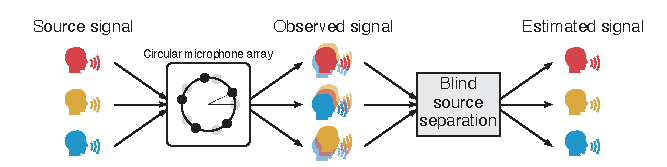
\includegraphics{figures/diagrams/bss.pdf}%
  \caption{Overview of blind source separation problem with a CMA.}%
  \label{fig:bss}
\end{figure}
Let us consider the BSS problem with a CMA that can be horizontally rotated as shown in \cref{fig:bss}.
Let $\Src$ and $\Mic$ be the numbers of sources and microphones, respectively.
We assume that the observed signal $\Obs _{\ft}$ is in the short-time Fourier transform (STFT) domain modeled as
\begin{equation}
  \Obs _{\ft} = \steer _{1,\ft} \sig _{1,\ft} + \dots + \steer _{\Src,\ft} \sig _{\Src,\ft} = \sum _{\src=1} ^{\Src} \steer _{\src,\ft} \sig _{\src,\ft},\label{eq:mix}
\end{equation}
where $\freq = 1, \dots, \Freq$ denotes the frequency bin index,
$\tframe = 1, \dots, \Tframe$ denotes the time frame index,
$\sig _{\src,\ft} \in \C\; (\src = 1, \dots, \Src)$ denotes the $\src$th source signal,
and $\steer _{\src,\ft} \in \C ^{\Mic}$ denotes the steering vector of the $\src$th source signal for each microphone.
Moreover, we here set the \emph{reference microphone} $\refmic = 1$ without the loss of generality.
In this case, each steering vector can be denoted as
\begin{equation}
  \steer _{\src,\ft} \coloneqq \begin{bmatrix} 1 & \str _{2,\src,\ft} & \dots & \str _{\Mic,\src,\ft} \end{bmatrix} ^{\top}\; (\src = 1, \dots, \Src).
\end{equation}
Under this definition, $\str _{\mic,\src,\ft} \; (\mic = 2, \dots, \Mic,\; \forall \src = 1, \dots, \Src)$ corresponds to the relative transfer function from the $\src$th source to the $\mic$th microphone, and thus each source signal $\sig _{1,\ft},\, \dots,\, \sig _{\Src,\ft}$ can be regarded as the \emph{source image} at the reference microphone.
Note that many BSS methods require a time-invariant mixing system $\steer _{\src,\freq}\; (\forall \src)$,
whereas, in this paper, steering vectors are time-variant $\steer _{\src,\ft}\; (\forall \src)$ to account for CMA rotation.
We aim to estimate source images at the reference microphone even when the CMA is rotated.
In the following, we assume that the rotation angle $\theta_t$ at each frame is known using another sensor, such as an angular acceleration sensor.

Next, we consider an online BSS problem analyzed using the model defined above.
We henceforth assume that the number of microphones of the CMA is equal to that of sources: $\Mic = \Src$.
\renewcommand{\Mic}{\Src}%
We aim to estimate demixing matrices and signals using only the currently and previously observed signals $\Obs _{\freq,1},\, \dots,\, \Obs _{\freq,\tframe}$:
\begin{align}
  \Demix _{\ft} &= \begin{bmatrix} \demix _{1,\ft} & \dots & \demix _{\Src,\ft} \end{bmatrix} ^{\hermite} \in \C ^{\Src \times \Mic}, \\
  \Est _{\ft} &= \Demix _{\ft} \Obs _{\ft} \in \C ^{\Src},\label{eq:bss:sep}
\end{align}
where $\Demix _{\ft}$ is the demixing matrix and $\Est _{\ft}$ is the estimated signal.

Unless otherwise specified, the indices $\freq,\, \tframe,$ and $\src$ always range from 1 to $\Freq, \Tframe,$ and $\Src$, respectively.
We omit the bounds of sets for these indices when they span the ranges.
${\{\Obs _{\ft}\}}_{\ft}$ denotes the set of $\Obs _{\ft}$ for all $\freq$ and $\tframe$, for example.
% \Cref{tab:notations} summarises the notations used in this paper.
% \begin{table}[t]
%   \centering
%   \caption{Notations}\label{tab:notations}
%   \begin{tabular}{lll}
%     \toprule
%       Symbol & Domain & Description \\
%     \midrule
%       % $\Mic$               & $\Z$                     & Number of microphones \\
%       $\Src$                               & $\Z$                     & Number of sources \\
%       $\steer _{\src,\ft}$                 & $\C ^{\Mic}$             & Steering vector \\
%       $\sig _{\src,\ft}$                   & $\C$                     & Source signal \\
%       $\Obs _{\ft}$                        & $\C^{\Mic}$              & Observed signal \\
%       $\Demix _{\ft}$                      & $\C^{\Src \times \Mic}$  & Demixing matrix \\
%       $\Est _{\ft}$                        & $\C^{\Mic}$              & Estimated signal \\
%       $\cov _{\src,\ft}$                   & $\C^{\Mic \times \Mic}$  & Covariance matrix \\
%       $\forget$                            & $\{\forget \in \R \mid 0 \leq \forget < 1\}$   & Forgetting factor \\
%       $\rotSpat _{\tframe}$                & $\R$                     & Spatial rotation angle \\
%       $\rotSmpl$                           & $\R$                     & Rotation angle coefficient on CMA \\
%       $\rotFra$                            & $\R$                     & Rotation time \\
%       $\rotMat (\rotSpat _{\tframe})$      & $\R ^{\Mic \times \Mic}$ & Rotation matrix \\
%       $\refpos{\Obs} _{\ft}$ & $\C^{\Mic}$ & Observes signal at reference position \\
%     \bottomrule
%   \end{tabular}
% \end{table}

\section{Conventional Methods}\label{sec:conventional}

\subsection{Batch AuxIVA}
As the basis of our work, we first summarize the \emph{batch} AuxIVA \cite{Ono:2011:WASPAA}.
In AuxIVA, we estimate \emph{time-invariant} demixing matrices ${\{\Demix _{\freq}\}} _{\freq}$ using all the time frames $\tframe = 1, \dots, \Tframe$ by minimizing the following objective function:
\begin{align}
  J _{\freq}(\Demix _{\freq}) &= \sum _{\src = 1} ^{\Src} \demix _{\src,\freq} ^{\hermite} \cov _{\src,\freq} \demix _{\src,\freq} ^{\nohermite} - \logdet{\Demix _{\freq}} ^2, \label{eq:obj:batch} \\
  \cov _{\src,\freq} &= \frac{1}{\Tframe} \sum _{\tframe = 1} ^{\Tframe} \weight(\var _{\src,\tframe}) \Obs _{\ft} ^{\nohermite} \Obs _{\ft} ^{\hermite}, \label{eq:cov:batch} \\
  \var _{\src,\tframe} &= \textstyle\sqrt{\sum _{\freq=1} ^{\Freq} \lvert \demix ^{\hermite} _{\src,\freq} \Obs ^{\nohermite}_{\ft} \rvert ^2} \label{eq:var:batch},
\end{align}
where
$\weight\colon \R _{>0} \to \R _{>0}$ is defined as $\weight(\var) = \cont ' (\var) / 2 \var$, with $\cont '(\var)$ being the first derivative of $\cont (\var)$ for $\var$
and $\cont(\var)$ is the contrast function derived from the probability density function of source signals.
In this paper, we assume that $\weight (\var) = \Freq/{\var ^2}$, which represents the time-varying Gaussian distribution \cite{Ono:2012:APSIPA}.
$\cov _{\src,\freq}$ is the \emph{weighted covariance matrix} of the observed signals.
One popular method of minimizing the objective function \eqref{eq:obj:batch} with respect to $\Demix _{\freq}$ includes \emph{iterative projection (IP)} \cite{Ono:2011:WASPAA}.
IP cyclically updates each row vector of the demixing matrix (\emph{demixing vector}) $\demix _{\src,\ft} ^{\hermite}\; (\src = 1, \dots, \Src)$ using the following update rule:
\begin{align}
  \demix _{\src,\freq} &\gets (\Demix _{\freq} \cov _{\src,\freq}) ^{-1} \eye _{\src} \label{eq:ip:proj}, \\
  \demix _{\src,\freq} &\gets \tfrac{{\demix _{\src,\freq}}}{{\sqrt{\demix _{\src,\freq} ^{\hermite} \cov _{\src,\freq} \demix _{\src,\freq}}}} \label{eq:ip:norm},
\end{align}
where $\eye _{\src} \in \R ^{\Src}$ is the canonical basis vector with the $\src$th element unity.
The estimated signal is estimated as $\Est _{\ft} = \Demix _{\freq} \Obs _{\ft}$.

\subsection{Online Auxiliary-Function-Based Independent Vector Analysis}\label{subsec:oiva}

Online AuxIVA (OIVA) \cite{Taniguchi:2014:HSCMA} is an extension of batch AuxIVA to an online algorithm.
In OIVA, the weighted covariance matrices are updated with the following incremental update rule as an approximation of \eqref{eq:cov:batch}:
\begin{align}
  \cov _{\src,\ft} &= \forget \cov _{\src,\ft[-1]} + (1 - \forget) \weight(\var _{\src,\tframe}) \Obs _{\ft} ^{\nohermite} \Obs _{\ft} ^{\hermite}, \label{eq:cov} \\
  \var _{\src,\tframe} &= \textstyle\sqrt{\sum _{\freq=1} ^{\Freq} \lvert \demix ^{\hermite} _{\src,\ft} \Obs ^{\nohermite}_{\ft} \rvert ^2} \label{eq:var},
\end{align}
where $\forget\; (0 \leq \forget < 1)$ is the forgetting factor.
With this incremental update rule, we can directly apply IP to estimating time-varying demixing matrices ${\{\Demix _{\ft}\}} _{\freq}$ at each time frame $\tframe$ by simply replacing $\demix _{\src,\freq},\, \cov _{\src,\freq}$ in \eqref{eq:ip:proj}, \eqref{eq:ip:norm} with $\demix _{\src,\ft},\, \cov _{\src,\ft}$.

We then estimate the signal using by \eqref{eq:bss:sep}.
The scale of the output estimated signal $\Est _{\ft}$ may be contaminated by the scale ambiguity problem.
To restore the scale ambiguity and obtain an estimated source image at the reference microphone,
we apply the following backprojection \cite{Murata:2001:NC} for postprocessing:
\begin{align}
  \proj{\Demix} _{\ft}
    &\gets
    \diag\left(\eye _{1} ^{\top} \Demix _{\ft} ^{-1} \right) \Demix _{\ft},
    \label{eq:pb:w}
    \\
  \Est _{\ft}
    &\gets
    \proj{\Demix }_{\ft} \Obs _{\ft},
    \label{eq:pb:y}
\end{align}
where $\diag(\cdot)$ is an operator for constructing a diagonal matrix with each of its elements equals the corresponding element of the given vector.
\Cref{alg:iva} summarizes the OIVA algorithm.
The online updates of $\cov _{\src,\ft}$ \eqref{eq:cov} enable OIVA to track the slow movement of sound sources or microphones progressively.
Nevertheless, it cannot promptly adapt to swift changes, which can happen in head rotation when wearing CMA on the head.
In this research, we aim to solve this problem.

\begin{algorithm}{Online AuxIVA (OIVA)}{iva}
  \textbf{Input:} ${\{\Obs _{\ft}\}} _{\ft}$, $ {\{\Demix _{\freq,0}\}} _{\freq}$, $ {\{\cov _{\src,\freq,0}\}} _{\src,\freq}$, $ \forget$\\
  \textbf{Output:} ${\{\Est _{\ft}\}} _{\ft}$
  \begin{pseudo}
    for $\tframe = 1, \dots, \Tframe$ \\+
      for $\freq = 1, \dots, \Freq$ \\+
        {$\Demix _{\ft}$} $\gets$ $\Demix _{\ft[-1]}$ \\-

      for $\itr = 1,\, \dots,\, \Itr$ \\+
        for $\src = 1,\, \dots,\, \Src$ \\+
          {$\var _{\src,\tframe}$} $\gets$ $\sqrt{\sum _{\freq = 1} ^{\Freq} \abs{\demix _{\src,\ft} ^{\hermite} \Obs _{\ft}} ^2}$ \ct{\eqref{eq:var}} \\
          for $\freq = 1, \dots, \Freq$ \\+
            {$\cov _{\src,\ft}    $} $\gets$ $\forget \cov _{\src,\ft[-1]} + (1 - \forget) \weight(\var _{\src,\tframe}) \Obs _{\ft} \Obs _{\ft} ^{\hermite}$ \ct{\eqref{eq:cov}} \\
            {$\demix _{\src,\ft}$} $\gets$ $\left(\Demix _{\ft} \cov _{\src,\ft}\right) ^{-1} \eye _{\src}$ \ct{\eqref{eq:ip:proj}} \\
            {$\demix _{\src,\ft}$} $\gets$ $\frac{\demix _{\src,\ft}}{\sqrt{\demix _{\src,\ft} ^{\hermite} \cov _{\src,\ft} \demix _{\src,\ft}}}$ \ct{\eqref{eq:ip:norm}} \\---

      for $\freq = 1, \dots, \Freq$ \\+
        \nf{$\proj{\Demix} _{\ft} \gets \diag\left(\eye _{1} ^{\top} \Demix _{\ft} ^{-1} \right) \Demix _{\ft}$} \ct{\eqref{eq:pb:w}}\\
        {$\Est _{\ft}$} $\gets$ $\proj{\Demix }_{\ft} \Obs _{\ft}$ \ct{\eqref{eq:pb:y}}
  \end{pseudo}
\end{algorithm}

\subsection{Sound Field Interpolation on Circular Microphone Array}
In this subsection, we briefly review the sound field interpolation method on a CMA, initially proposed in \cite{Wakabayashi:2021:ICASSP,Wakabayashi:2023:ASLP}.
Let $\sfcma (\rotCoor)$ be a continuous sound pressure on the circumference of a circle at a spatial angle $\rotCoor \in \interval[open right,soft open fences]{0}{2\pi}$, as shown in \cref{fig:sfi}.
Then, we observe a sound field with $\Mic$ microphones distributed on the circle at even intervals.
The $\mic$th observed signal is denoted as
\begin{equation}
  \sfcma _{\mic} = \sfcma \left(2\pi \frac{\mic}{\Mic}\right),\; (\mic = 0, \dots, \Mic - 1).%
  \label{eq:sfi:model}
\end{equation}
In other words, we regard the observations of the sound field with a CMA as the discretizations of that along an angle on the circumference $\rotCoor$.
We assume that this spatial sampling by the CMA satisfies Shanon's sampling theorem, \emph{i.e.}, $\sfcma (\rotCoor)$ contains no frequency components higher than half of the sampling frequency on the circumference of the circle.
If the CMA is rotated by a spatial angle $\rotSpat \in \R$, we can regard its observation as the $\rotSmpl$-sample shift of $\sfcma _{\mic}$ where $\rotSmpl = \frac{\Mic}{2\pi} \rotSpat$;
\begin{equation}
  \sfcma \left(\frac{2\pi}{\Mic} \mic + \rotSpat \right)%
  \coloneqq
  \sfcma _{\mic + \rotSmpl}.
  \label{eq:sfi:shift:obs}
\end{equation}
\begin{figure}[t]
  \centering
  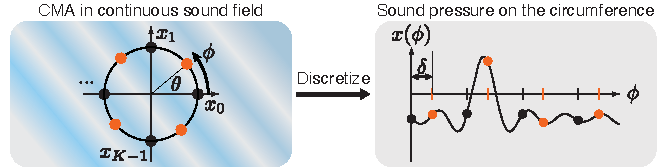
\includegraphics{figures/diagrams/sfi.pdf}
  \caption{%
    Concept of sound field interpolation on a CMA.
    The left figure shows the CMA in a continuous sound field (six microphones in this example).
    Each black dot is a microphone at the reference position, and each gray dot is a microphone at the rotated position.
    Background colors indicate the sound pressure of a plane wave.
    The right side shows the sound pressure along the circumference.
  }%
  \label{fig:sfi}
\end{figure}

Next, we formulate a sound field interpolation problem with the model above.
We define the $\Mic$-point spatial discrete Fourier transform (DFT) of $\sfcma _{\mic}$ and its inverse transform as
\begin{align}
  \dft _{\Src} [\sfcma _{\mic}] &= \sum _{\mic \in \SRC} \sfcma _{\mic} \twid ^{-\mic\src} \coloneqq \Sfcma _{\src},\\
  \dft _{\Src} ^{-1} [\Sfcma _{\src}] &= \frac{1}{\Mic} \sum _{\src \in \SRC} \Sfcma _{\src} \twid ^{\mic\src},%\\
\end{align}
where $\twid \coloneqq \exp (j \frac{2\pi}{\Mic})$ is a twidle factor of the $\Mic$-point DFT, $j$ is the imaginary unit, and $\SRC$ is an index set defined as
\begin{align}
  \SRC &=
  \begin{cases}
    \left\{-\frac{\Src}{2} + 1, -\frac{\Src}{2} + 2, \dots, \frac{\Src}{2}\right\} & \text{($\Src$ is even)}, \\
    \left\{-\frac{\Src - 1}{2}, -\frac{\Src - 1}{2} + 1, \dots, \frac{\Src - 1}{2}\right\} & \text{($\Src$ is odd)}.
  \end{cases}
\end{align}
As is well known, for the shift theorem of DFT, the following equation is satisfied for any integers $d$:
\begin{equation}
  \dft _{\Src} [\sfcma _{\mic + d}] = \Sfcma _{\src} \twid ^{d \src}.%
  \label{eq:sfi:shift:int}
\end{equation}
Although \eqref{eq:sfi:shift:int} does not hold strictly for real numbers, we assume that the following equation holds approximately for a real number $\rotSmpl$:
\begin{equation}
  \dft _{\Src} [\sfcma _{\mic + \rotSmpl}] = \Sfcma _{\src} \twid ^{\rotSmpl \src}.%
  \label{eq:sfi:shift:dft}
\end{equation}
From these assumptions, we have
\begin{align}
  \sfcma _{\mic + \rotSmpl} &= \dft _{\Src} ^{-1} \left[\Sfcma _{\src} \twid ^{\rotSmpl \src}\right], \\
                            &= \frac{1}{\Mic} \sum _{\src \in \SRC} \left(\Sfcma _{\src}\twid ^{\rotSmpl\src} \right) \twid ^{\mic\src}, \\
                            &= \frac{1}{\Mic} \sum _{\src \in \SRC} \left(\sum _{n=0} ^{\Mic - 1} \sfcma _{n} \twid ^{-n\src}\right) \left( \twid ^{(\rotSmpl + \mic)\src} \right), \\
                            &= \sum _{\dum = 0} ^{\Mic - 1} \sfcma _{\dum} \left( \frac{1}{\Mic} \sum _{\src \in \SRC} \twid ^{(\rotSmpl + \mic - \dum)\src} \right)
                            \coloneqq \sum _{\dum = 0} ^{\Mic - 1} \sfcma _{\dum} \rotmat _{\mic, \dum}(\rotSmpl) \label{eq:sfi:elem}.
\end{align}
The coefficient $\rotmat _{\mic,\dum}(\rotSmpl)$ is calculated as
\begin{align}
  \rotmat _{\mic,\dum}(\rotSpat)
  &=
    \begin{cases}
      \displaystyle\frac{\twid ^{- \rotIdx (\frac{\Mic}{2} - 1) }}{\Mic} \frac{1 - \twid ^{\rotIdx \Mic}}{1 - \twid ^{\rotIdx}}\\[1em]
      \displaystyle\frac{\twid ^{- \rotIdx \frac{\Src - 1}{2}}}{\Mic} \frac{1 - \twid ^{\rotIdx \Mic}}{1 - \twid ^{\rotIdx}}
    \end{cases}
  =
    \begin{cases}
      \displaystyle \frac{\sinc{(\rotIdx)}}{\sinc{\left(\rotIdx / \Mic\right)}} \twid ^{\frac{\rotIdx}{2}} & (\text{$\Mic$ is even}),\\[1em]
      \displaystyle \frac{\sinc{(\rotIdx)}}{\sinc{\left(\rotIdx / \Mic\right)}} & (\text{$\Mic$ is odd}),
    \end{cases}\label{eq:rot:sinc}
\end{align}
where $\rotIdx =\rotSmpl + \mic - \dum; (\mic, \dum = 0, \dots, \Mic - 1)$ \cite{Wakabayashi:2023:ASLP}.
\eqref{eq:rot:sinc} is an alternative expression for (3) in \cite{Wakabayashi:2023:ASLP}.
See Section II of \cite{Wakabayashi:2023:ASLP} for the detailed derivation.

The above relationship also holds in the frequency domain.
Let us define the following vector:
\begin{align}
  \bm{\sfcma} &= \begin{bmatrix} \sfcma _{0} & \dots & \sfcma _{\Mic - 1} \end{bmatrix} ^{\top}, \\
  \bm{\sfcma} _{\rotSmpl} &= \begin{bmatrix} \sfcma _{0+\rotSmpl} & \dots & \sfcma _{(\Mic - 1)+\rotSmpl} \end{bmatrix} ^{\top}.
\end{align}
From \eqref{eq:sfi:elem}, we have
\begin{equation}
  \bm{\sfcma} _{\rotSmpl}
  =
  \begin{bmatrix}
    \rotmat _{0, 0}(\rotSpat) & \dots & \rotmat _{0, \Mic - 1}(\rotSpat) \\
    \vdots & \ddots & \vdots \\
    \rotmat _{\Mic - 1, 0}(\rotSpat) & \dots & \rotmat _{\Mic - 1, \Mic - 1}(\rotSpat)
  \end{bmatrix}
  \bm{\sfcma}
  \coloneqq
  \rotMat (\rotSpat) \bm{\sfcma},
  \label{eq:rotmat}
\end{equation}
where $\rotMat (\rotSpat) \in \C ^{\Mic\times\Mic}$ is the \emph{rotation matrix}.
By definition, $\rotMat (\rotSpat)$ is obviously a unitary matrix: $\rotMat ^{-1} (\rotSpat) = \rotMat ^{\hermite} (\rotSpat)$.
Next, let $\bm{\Sfcma}$ be its DFT defined as $\begin{bmatrix} \Sfcma _{0} & \dots & \Sfcma _{\Mic - 1}\end{bmatrix} ^{\top} = \bm{F} \bm{\sfcma}$, where $\bm{F}$ is a $\Src$-point DFT matrix.
By using these expressions, we can diagonalize $\rotMat (\rotSpat)$ as $\bm{F}^{\hermite} \rotMat (\rotSpat) \bm{F}$ since $\rotMat (\rotSpat)$ is a unitary matrix.
Therefore, the relationship between $\bm{\Sfcma}$ and $\bm{\Sfcma} _{\rotSmpl}$ can be expressed as $\bm{X} _{\rotSmpl} = \rotMat (\rotSpat) \bm{X}$,
because $\bm{\sfcma} _{\rotSmpl} = \bm{F}^{\hermite} \rotMat (\rotSpat) \bm{F} \bm{\sfcma}$.

In the STFT domain, we consider a situation where a CMA is rotated by degree $\rotSpat _{\tframe}$ at the time frame $\tframe$, and let $\refpos{\Obs} _{\ft}$ be the observed signal recorded without CMA rotation (\emph{reference position}).
By using the expression above, we assume that the observed signal with CMA rotation $\Obs _{\ft}$ is expressed as the following linear approximation:
\begin{equation}
  \refpos{\Obs} _{\ft} = \rotMat ^{-1} (\rotSpat _{\tframe}) \Obs _{\ft}.
\end{equation}
As mentioned in the previous section, note that $\rotSpat _{\tframe}$ must be known using another sensor, such as an angular acceleration sensor, or estimated from the acoustic observation itself \cite{Lian:2021:APSIPA}.

\section{Proposed Method}\label{sec:proposed}

% We propose two types of algorithms; sound field interpolation based online AuxIVA.
% \Cref{fig:system} shows the system architecture of our proposed methods.
% \begin{figure}[h]
%   \begin{minipage}[t]{\linewidth}
%     \centering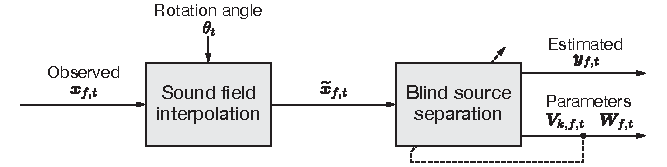
\includegraphics{figures/diagrams/sfiiva-o.pdf}\subcaption{SFIIVA-Obs}\label{fig:sfiiva-o}
%   \end{minipage}
%   \begin{minipage}[t]{\linewidth}
%     \centering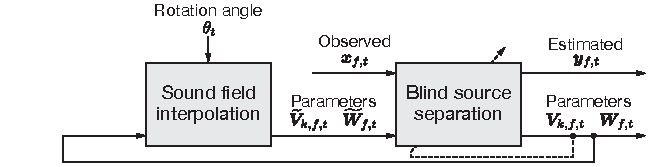
\includegraphics{figures/diagrams/sfiiva-m.pdf}\subcaption{SFIIVA-Par}\label{fig:sfiiva-m}
%   \end{minipage}
%   \caption{System diagram of proposed algorithms.}
%   \label{fig:system}
% \end{figure}

% TODO: illustration for difference between SFIIVA-O and SFIIVA-M
\subsection{SFI-based Online AuxIVA with Transformation of Latest Observation}

In the beamforming that is robust against the self-rotation proposed in \cite{Wakabayashi:2023:ASLP},
the signals observed by the CMA with angle $\theta_t$ are transformed frame by frame to what would have been observed at the reference position,
namely, at the angle $\theta=0$, using SFI, and then the beamforming is applied to the transformed signals.

To make OIVA robust against self-rotation, we first consider a similar approach to \cite{Wakabayashi:2023:ASLP} in this subsection.
In this method, we simply apply the transformation using SFI to the latest observation, \emph{i.e.},
\begin{align}
  \refpos{\Obs} _{\ft} &\gets \rotMat ^{\hermite} (\rotSpat _{\tframe}) \Obs _{\ft},
  \label{eq:sfi:obs}
\end{align}
and the online update of the weighted covariance matrix $\cov _{\src,\ft}$ is performed using the transformed signal $\refpos{\Obs} _{\ft}$ such as
\begin{align}
  \cov _{\src,\ft}\gets \forget \cov _{\src,\ft[-1]} + (1 - \forget) \weight(\var _{\src,\tframe}) \refpos{\Obs} _{\ft} \refpos{\Obs} _{\ft} ^{\hermite}.
  \label{eq:cov:rot}
\end{align}
The demixing matrices $\Demix _{\ft}$ are estimated by using these weighted covariance matrices $\cov _{\src,\ft}$ similarly to OIVA.
\Cref{alg:sfiva-o} summarizes OIVA using this approach, and \cref{fig:sfiiva-m} shows the system diagram.

Assuming that a CMA rotates only once at a specific time frame $\tframe$, we analyze how the proposed method, as given in \cref{eq:cov:rot}, differs from the original formula in \cref{eq:cov}.
In \cref{eq:cov}, the value of $\cov _{\src,\ft}$ is updated online.
However, since the angle of the CMA differs between the time frames $\tframe - 1$ and $\tframe$, the blending of $\cov _{\src,\ft[-1]}$, which holds information before the rotation, and $\Obs _{\ft}$, which holds information after the rotation, leads to an inaccurate estimation of the demixing matrix $\Demix _{\ft}$.
If the CMA does not rotate further after the time frame $\tframe$,
the observation information before the rotation is gradually diminished, and
$\cov _{\src,\ft}$ and $\Demix _{\ft}$ are expected to slowly converge to their values associated with the postrotation position of CMA.
However, this convergence is expected to take time.
In contrast, in \cref{eq:cov:rot}, all observed signals are translated into the observation at the reference position.
Thus, even if the CMA rotates at the time frame $\tframe$, there is no substantial discrepancy between $\cov _{\src,\ft[-1]}$ and $\refpos{\Obs} _{\ft}$, and the effect of the rotation on the estimation of the demixing matrix $\Demix _{\ft}$ is expected to be markedly reduced.

Note that the separated signals obtained by this approach are the source images at the reference microphone of the CMA with the reference angle.
Since the position of the reference microphone is fixed in the space regardless of the CMA rotation, this causes problems in some practical applications.
For example, in hearing aid applications or virtual/augmented reality (VR/AR) applications with a head-mounted display, it is desired to present a separated signal with the source localization sensation.
For this purpose, we should estimate the source images on the reference microphone of the CMA rotated together with the head.

\begin{algorithm}{SFI-based Online AuxIVA using Transformation of Latest Observation (\SFIIVAo)}{sfiva-o}
  \textbf{Input:} ${\{\Obs _{\ft}\}} _{\ft}$, ${\{\Demix _{\freq,0}\}} _{\freq}$, ${\{\cov _{\src,\freq,0}\}} _{\src,\freq}$, $\forget$, ${\{\rotSpat _{\tframe}\}} _{\tframe}$ \\
  \textbf{Output:} ${\{\Est _{\ft}\}} _{\ft}$
  \begin{pseudo}
    for $\tframe = 1,\, \dots,\, \Tframe$ \\+
      for $\freq = 1, \dots, \Freq$ \\+
        $\refpos{\Obs} _{\ft} \gets \rotMat ^{\hermite} (\rotSpat _{\tframe}) \Obs _{\ft}$ \ct{\eqref{eq:sfi:obs}} \\
        {$\Demix _{\ft}$} $\gets$ $\Demix _{\ft[-1]}$ \\-
      for $\itr = 1,\, \dots,\, \Itr$ \\+
        for $\src = 1,\, \dots,\, \Src$ \\+
          {$\var _{\src,\tframe}$} $\gets$ $\sqrt{\sum _{\freq = 1} ^{\Freq} \abs{\demix _{\src,\ft} ^{\hermite} \refpos{\Obs} _{\ft}} ^2}$ \ct{\eqref{eq:var}} \\
          for $\freq = 1, \dots, \Freq$ \\+
            {$\cov _{\src,\ft}    $} $\gets$ $\forget \cov _{\src,\ft[-1]} + (1 - \forget) \weight(\var _{\src,\tframe}) \refpos{\Obs} _{\ft} \refpos{\Obs} _{\ft} ^{\hermite}$ \ct{\eqref{eq:cov:rot}} \\
            {$\demix _{\src,\ft}$} $\gets$ $\left(\Demix _{\ft} \cov _{\src,\ft}\right) ^{-1} \eye _{\src}$ \ct{\eqref{eq:ip:proj}} \\
            {$\demix _{\src,\ft}$} $\gets$ $\frac{\demix _{\src,\ft}}{\sqrt{\demix _{\src,\ft} ^{\hermite} \cov _{\src,\ft} \demix _{\src,\ft}}}$ \ct{\eqref{eq:ip:norm}} \\---

      for $\freq = 1, \dots, \Freq$ \\+
        \nf{$\proj{\Demix} _{\ft} \gets \diag\left(\eye _{1} ^{\top} \Demix _{\ft} ^{-1} \right) \Demix _{\ft}$} \ct{\eqref{eq:pb:w}}\\
        {$\Est _{\ft}$} $\gets$ $\proj{\Demix }_{\ft} \refpos{\Obs} _{\ft}$ \ct{\eqref{eq:pb:y}}
  \end{pseudo}
\end{algorithm}

\subsection{SFI-based Online AuxIVA with Transformation of Pre-update Demixing and Weighted Covariance Matrices}\label{subsec:proposed:sfiivam}

In this subsection, we propose another online BSS that is robust against CMA rotation and outputs the source image at the latest reference microphone position frame by frame.
As discussed in the previous section, the mismatch between $\cov _{\src,\ft[-1]}$ and $\Obs _{\ft}$ causes a problem.
In the previous approach, we transform $\Obs _{\ft}$ to what it should be at the reference position of the CMA.
In this subsection, we consider another approach: transforming $\cov _{\src,\ft[-1]}$ to what it should be at the latest position of the CMA.

First, we discuss the parameter transformation in a \emph{time-invariant} case for simplicity.
In this case, demixing matrices $\Demix _{\freq}$ and weighted covariance matrices $\cov _{\src,\freq}$ are independent of the time frame $\tframe$.
Let $\Obs _{\ft}$ and $\refpos{\Obs}_{\ft}$ be observations if the angle of the CMA is fixed at $\rotSpat _1$ and $\rotSpat _2$, respectively.
If the approximation of SFI is satisfied, $\Obs _{\ft}$ and $\refpos{\Obs} _{\ft}$ hold the following relation:
\begin{equation}
  \refpos{\Obs} _{\ft} = \rotMat (\Delta\rotSpat)\Obs _{\ft},
\end{equation}
where $\Delta\rotSpat = \rotSpat _2 - \rotSpat _1$.
From this, we have the estimated signal $\Est _{\ft}$ as
\begin{align}
  \Est _{\ft} &= \Demix _{\freq} \Obs _{\ft}, \\
              &= \Demix _{\freq} \rotMat ^{\hermite} (\Delta\rotSpat) \refpos{\Obs} _{\ft} \coloneqq \refpos{\Demix} _{\freq} \refpos{\Obs} _{\ft}, \label{eq:rt:demix:batch}
\end{align}
where $\Demix_{\freq}$ and $\refpos{\Demix} _{\freq}$ are time-invariant demixing matrices
for $\Obs _{\ft}$ and $\refpos{\Obs} _{\ft}$, respectively.
Therefore,
\begin{align}
  \refpos{\Demix} _{\freq} = \Demix _{\freq} \rotMat ^{\hermite} (\Delta\rotSpat). \label{eq:demix:refpos}
\end{align}
Similarly, the time-invariant weighted covariance matrix $\cov_{\src,\freq}$ estimated using $\Obs_{\ft}$ is calculated as
\begin{equation}
  \cov _{\src,\freq} = \expct  _{\tframe} \left[\weight (\var _{\src,\tframe}) \Obs _{\ft} \Obs _{\ft} ^{\hermite}\right],
\end{equation}
where $\expct _{\tframe}\left[\bm{A} _{\tframe}\right]$ is the expectation operation for the random variable matrix $\bm{A}_{\tframe}$ with respect to the time frame $\tframe$.
We rewrite the weighted covariance matrix ${\cov} _{\src,\freq}$ of $\Obs _{\ft}$ using $\refpos{\cov} _{\src,\freq}$ as
\begin{align}
  \refpos{\cov} _{\src,\freq} &= \expct  _{\tframe} \left[\weight (\var _{\src,\tframe}) \refpos{\Obs} _{\ft} \refpos{\Obs} _{\ft} ^{\hermite}\right], \\
                     &= \expct  _{\tframe} \left[\weight (\var _{\src,\tframe}) \rotMat (\Delta\rotSpat) {\Obs} _{\ft} {\Obs} _{\ft} ^{\hermite} \rotMat ^{\hermite} (\Delta\rotSpat)\right], \\
                     &= \rotMat (\Delta\rotSpat)\; \expct  _{\tframe} \left[\weight (\var _{\src,\tframe}) {\Obs} _{\ft} {\Obs} _{\ft} ^{\hermite} \right] \rotMat ^{\hermite} (\Delta\rotSpat), \\
                     &= \rotMat (\Delta\rotSpat) {\cov} _{\src,\freq} \rotMat ^{\hermite} (\Delta\rotSpat). \label{eq:cov:refpos:batch}
\end{align}

Although $\cov _{\src,\ft}$ and $\Demix _{\ft}$ are estimated online in OIVA,
we use these variable transformations written in \eqref{eq:demix:refpos} and \eqref{eq:cov:refpos:batch} for the preprocessing of their update to compensate for the CMA rotation such as
\begin{align}
  \refpos{\Demix} _{\ft[-1]} &\gets \Demix _{\ft[-1]} \rotMat ^{\hermite} (\Delta \rotSpat _{\tframe}), \label{eq:sfiiva:demix} \\
  \refpos{\cov} _{\src,\ft[-1]} &\gets \rotMat (\Delta\rotSpat _{\tframe}) \cov _{\src,\ft[-1]} \rotMat ^{\hermite} (\Delta\rotSpat _{\tframe}), \label{eq:sfiiva:cov}
\end{align}
where $\Delta\rotSpat _{\tframe} = \rotSpat _{\tframe} - \rotSpat _{\tframe - 1}$.
This method preserves the observation as is and transforms the intermediate variables as $\Demix _{\ft[-1]}$ and $\cov _{\src,\ft[-1]}$ instead;
thus, the source image at the latest CMA position can be estimated, which is an advantage of this algorithm.
Furthermore, the angle of the CMA is supposed to be measured by integrating angular accelerometers, which can introduce bias errors.
In this case, the method described in the previous subsection continues to have errors in the transformation of the observations to those at the reference position.
On the other hand, in the method described in this subsection, the error included in the transformation of $\Demix _{\ft}$ and $\cov _{\src,\ft}$ should disappear with online updates.
This is another advantage of this approach. We will show this in an experiment to be described later.
The entire algorithm is summarized as \cref{alg:sfiva-m}, and \cref{fig:sfiiva-m} shows the system diagram of our approach.

\begin{algorithm}{SFI-based Online AuxIVA with Transformation of Pre-update Demixing and Weighted Covariance Matrices (\SFIIVAm)}{sfiva-m}
  \textbf{Input:} ${\{\Obs _{\ft}\}} _{\ft}$, ${\{\Demix _{\freq,0}\}} _{\freq}$, ${\{\cov _{\src,\freq,0}\}} _{\src,\freq}$, $\forget$, ${\{\rotSpat _{\tframe}\}} _{\tframe}$ \\
  \textbf{Output:} ${\{\Est _{\ft}\}} _{\ft}$
  \begin{pseudo}

    for $\tframe = 1,\, \dots,\, \Tframe$ \\+
      $\varDelta \rotSpat _{\tframe} \gets \rotSpat _{\tframe} - \rotSpat _{\tframe - 1}$ \\
      for $\freq = 1, \dots, \Freq$ \\+
        {$\Demix _{\freq,\tframe}$} $\gets$ $\Demix _{\freq,\tframe - 1} \rotMat ^{\hermite} (\varDelta\rotSpat _{\tframe})$ \ct{\eqref{eq:sfiiva:demix}} \\
        for $\src = 1,\, \dots,\, \Src$ \\+
          {$\refpos{\cov} _{\src,\ft[-1]}$} $\gets$ $\rotMat (\varDelta\rotSpat _{\tframe}) \cov _{\src,\ft[-1]} \rotMat ^{\hermite} (\varDelta \rotSpat _{\tframe})$ \ct{\eqref{eq:sfiiva:cov}} \\--
      for $\itr = 1,\, \dots,\, \Itr$ \\+
        for $\src = 1,\, \dots,\, \Src$ \\+
          {$\var _{\src,\tframe}$} $\gets$ $\sqrt{\sum _{\freq = 1} ^{\Freq} \abs{\demix _{\src,\ft} ^{\hermite} \Obs _{\ft}} ^2}$ \ct{\eqref{eq:var}} \\
          for $\freq = 1, \dots, \Freq$ \\+
            {$\cov _{\src,\ft}    $} $\gets$ $\forget \refpos{\cov} _{\src,\ft[-1]} + (1 - \forget) \weight(\var _{\src,\tframe}) \Obs _{\ft} \Obs _{\ft} ^{\hermite}$ \\
            {$\demix _{\src,\ft}$} $\gets$ $\left(\Demix _{\ft} \cov _{\src,\ft}\right) ^{-1} \eye _{\src}$ \ct{\eqref{eq:ip:proj}} \\
            {$\demix _{\src,\ft}$} $\gets$ $\frac{\demix _{\src,\ft}}{\sqrt{\demix _{\src,\ft} ^{\hermite} \cov _{\src,\ft} \demix _{\src,\ft}}}$ \ct{\eqref{eq:ip:norm}} \\---

      for $\freq = 1, \dots, \Freq$ \\+
        \nf{$\proj{\Demix} _{\ft} \gets \diag\left(\eye _{1} ^{\top} \Demix _{\ft} ^{-1} \right) \Demix _{\ft}$} \ct{\eqref{eq:pb:w}}\\
        {$\Est _{\ft}$} $\gets$ $\proj{\Demix }_{\ft} \Obs _{\ft}$ \ct{\eqref{eq:pb:y}}
  \end{pseudo}
\end{algorithm}

\begin{figure}[t]
  \centering
  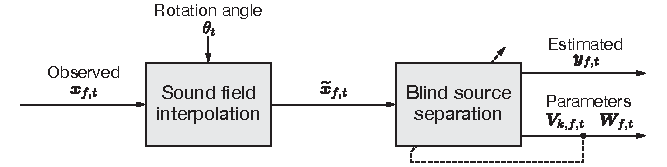
\includegraphics{figures/diagrams/sfiiva-o.pdf}
  \caption{System diagram of proposed \SFIIVAo{}}%
  \label{fig:sfiiva-o}
\end{figure}
\begin{figure}[t]
  \centering
  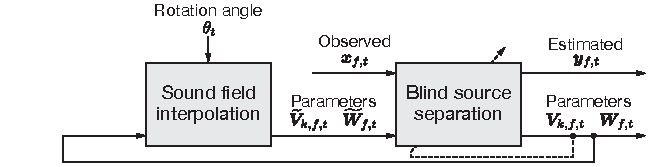
\includegraphics{figures/diagrams/sfiiva-m.pdf}
  \caption{System diagram of proposed \SFIIVAm{}}%
  \label{fig:sfiiva-m}
\end{figure}

\section{Experimental Validation}\label{sec:experiment}
% Although OIVA can track slow microphone movements, its convergence performance highly depends on the forgetting factor.
% Furthermore, ICA-based BSS methods do not change the results even if the observed signals are ``remixed.''
% For example, the same output is obtained by inputting the 2-channel observed signals $x_1$ and $x_2$ as $x_1 + x_2$ and $x_1 - x_2$.
% Since the transformation of the observed signals by the SFI can also be interpreted as a kind of ``remixing,''
% the separation performance is expected to remain the same regardless of whether or not the SFI is performed before or after the CMA rotation.
% However, it has been reported that SFI improves the separation performance \cite{Nakashima:2022:ASJ:A}.
In this section, we confirm with our experimental results how much SFI contributes to BSS and discuss the difference in the location of the source image due to the SFI.
Henceforth, we assume that the CMA was instantaneously rotated at the angle $\rotSpat$ at the time frame $\rotFra$.

\subsection{Setup}

Simulation experiments with large random synthesized datasets were conducted to evaluate the performance of BSS under a situation where a CMA rotates.
The datasets consisted of 100 samples, and each sample simulated observed signals with five source signals with a five-channel CMA using the image source method \cite{Allen:1979:JASA}.
As the source signals, we used the speech signals of five speakers (\texttt{jvs001}, \texttt{jvs002,} $\hdots$, \texttt{jvs005}) from the JVS dataset \cite{Takamichi:2019:arxiv}.
In this experiment, the utterances included in \texttt{parallel100} were randomly concatenated for each speaker.
The length was \SI{60}{\second}, and the sampling frequency was resampled from \SI{24}{\kilo\hertz} to \SI{16}{\kilo\hertz}.
The reverberation time was approximately \SI{100}{\milli\second}.
A CMA with $\Src = 5$ channels and a radius of \SI{2}{\centi\metre} was placed at the center of the room.
Each source was randomly placed at least \SI{1}{\metre} from the center of the CMA and within an angle ranging from $\frac{360}{\Src} \src$ to $\frac{360\si{\degree}}{\Src} (\src - 1) + \frac{180\si{\degree}}{\Src}\; (\src = 1, \dots, \Src)$.
\Cref{fig:layout:exp} illustrates the range of sources' placements and their examples.
To simulate the instant rotation of the CMA, the source images were generated when the CMA was rotated \SI{40}{\degree} counter-clockwise from the horizontal axis and was joined together at 0--30 \si{\second} and 30--60 \si{\second} intervals.
Note that the rotation angle and time are given in an oracle manner.
STFT was performed on the observed signals with a frame length of 4096 points, a shift length of 2048 points, and a Hamming window.
The scale of the output signal was restored by backprojection as shown in \cref{alg:iva}, with the reference microphone as microphone 1.
The separation performance was evaluated by the scale-invariant signal-to-distortion ratio (SI-SDR) \cite{LeRoux:2019:ICASSP} and its improvement (SI-SDR improvement; SI-SDRi).
The reference signal for the SI-SDR was the source image recorded with a rotated CMA.
\begin{figure}[t]
  \centering
  \begin{minipage}[t]{.45\linewidth}
    \centering
    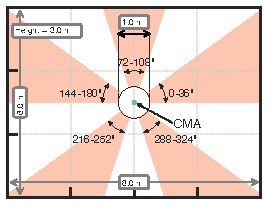
\includegraphics[width=\columnwidth]{figures/room_layout_range.pdf}
    \subcaption{Five sources are randomly placed in each orange-shaded area.}%
    \label{fig:layout:range}
  \end{minipage}
  \hspace{.05\linewidth}
  \begin{minipage}[t]{.45\linewidth}
    \centering
    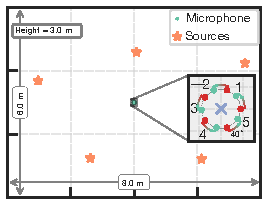
\includegraphics[width=\columnwidth]{figures/room_layout_one.pdf}
    \subcaption{Example of sources and microphones placement.}%
    \label{fig:layout:one}
  \end{minipage}
  \caption{%
    Room layout. The center of CMA is placed at $(\SI{4.0}{\metre}, \SI{3.0}{\metre})$ in the room with the radius of \SI{2}{\centi\metre}. CMA was rotated \SI{40}{\degree} counter-clockwise at \SI{30}{\second}.
    In the zoomed plot of (b), red dots represent the microphones at the position before rotation, green dots represent the position after rotation, and the cross lines in the middle represent the center of CMA.
  }%
  \label{fig:layout:exp}
\end{figure}

The initial values for demixing and weighted covariance matrices were
$\Demix _{\freq,0} = \Eye\; (\forall \freq)$ and $\cov _{\src,\freq,0} = 10^{-3} \times \Eye\; (\forall \src, \freq)$, respectively, where $\Eye$ is the $\Src$-dimensional identity matrix.
We set the number of iterations in each time frame in \cref{alg:iva} $\Itr$ to 5.
We ran experiments using various forgetting factors $\forget = 0.9, 0.95, 0.98, \text{and} 0.99$,
which were chosen so that the approximate number of frames $\frac{1}{1 - \forget} =$ 10, 20, 50, and 100, respectively.
To increase numerous stability for the implementation of OIVA,
we applied the following ad-hoc normalization $\cov _{\src,\ft} \gets \cov _{\src,\ft} + 10 ^{-3} \times \Eye$ after updates using \eqref{eq:cov}.
We compared the following four methods:
\begin{description}
  \item[\NaiveIVA] OIVA described in \cref{subsec:oiva} as a baseline.
  \item[\ResetIVA] Re-initialize the weighted covariance and demixing matrices when the CMA was rotated:
      $\Demix _{\freq,\rotFra - 1} \gets \Eye, \; \cov _{\src,\freq,\rotFra - 1} \gets \varepsilon \Eye.$
  \item[\SFIIVAo] Apply SFI to the latest observation and estimate the source image at the fixed position (see \Cref{alg:sfiva-o}).
  \item[\SFIIVAm] Apply SFI to the weighted covariance and demixing matrices as parameter transformation and estimate the source image at the position rotated with CMA (see \Cref{alg:sfiva-m}).
\end{description}

\subsection{Source Separation Performance}
\subsubsection{Noiseless Environments}

As an initial experiment to verify the efficacy of the proposed methods, we first investigated source separation performance under a noise-less environment.
\Cref{fig:plot:line} shows the SI-SDRi every \SI{1}{\second} averaged over samples and channels.
As shown in \cref{fig:plot:line}, the result of forgetting factor $\forget$ of 0.9 showed faster tracking to the CMA rotation than the other results.
This is because the closer the forgetting factor $\forget$ to 0, the smaller the contribution of past signals.
However, the final performance was lower with no significant difference between the four methods and saturated after a sufficient time.
\Cref{fig:plot:box} shows the SI-SDRi averaged over samples and channels immediately after CMA rotation and after a sufficient time has elapsed.
Overall, \NaiveIVA{} and \ResetIVA{} showed a performance drop immediately after CMA rotation and improved again with time.
\ResetIVA{} has the lowest performance before CMA rotation among all forgetting factors, which worsens as the forgetting factor approaches 1.
In contrast, the proposed \SFIIVAm{} and \SFIIVAo{} methods performed better immediately after the CMA rotation than the others.
Between \SFIIVAm{} and \SFIIVAo{}, \SFIIVAm{} performed slightly better,
which may be due to the fact that \SFIIVAo{} estimates the source image at the reference microphone,
whereas the reference signal for SI-SDR evaluation was the source image at the reference position.
\begin{figure}[t]
  \centering
  \begin{minipage}[t]{.45\textwidth}
    \centering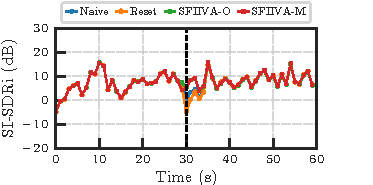
\includegraphics{figures/plots/clean/line_900.pdf}\subcaption{$\forget = 0.9  $}\label{fig:plot:line:900}
  \end{minipage}
  \hspace{.05\textwidth}
  \begin{minipage}[t]{.45\textwidth}
    \centering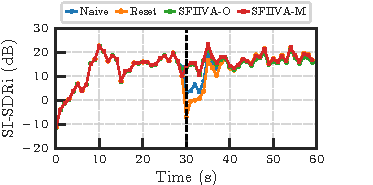
\includegraphics{figures/plots/clean/line_950.pdf}\subcaption{$\forget = 0.95 $}\label{fig:plot:line:950}
  \end{minipage}

  \begin{minipage}[t]{.45\textwidth}
    \centering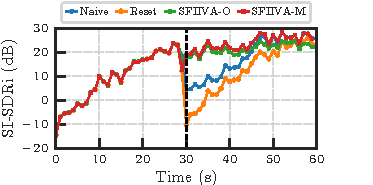
\includegraphics{figures/plots/clean/line_980.pdf}\subcaption{$\forget = 0.98 $}\label{fig:plot:line:980}
  \end{minipage}
  \hspace{.05\textwidth}
  \begin{minipage}[t]{.45\textwidth}
    \centering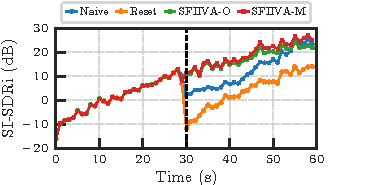
\includegraphics{figures/plots/clean/line_990.pdf}\subcaption{$\forget = 0.99 $}\label{fig:plot:line:990}
  \end{minipage}
  \caption{SI-SDR improvements (SI-SDRi) every \SI{1}{\second} under noiseless environments.}%
  \label{fig:plot:line}
\end{figure}

\begin{figure}
  \centering
  \begin{minipage}[t]{.45\textwidth}
    \centering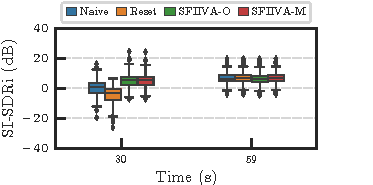
\includegraphics{figures/plots/clean/box_900.pdf}\subcaption{$\forget = 0.9  $}\label{fig:plot:box:900}
  \end{minipage}
  \hspace{.05\textwidth}
  \begin{minipage}[t]{.45\textwidth}
    \centering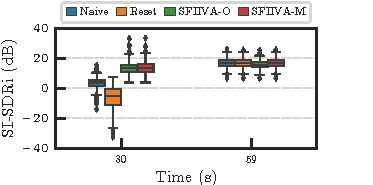
\includegraphics{figures/plots/clean/box_950.pdf}\subcaption{$\forget = 0.95 $}\label{fig:plot:box:950}
  \end{minipage}

  \begin{minipage}[t]{.45\textwidth}
    \centering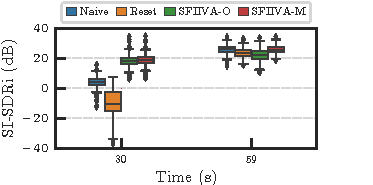
\includegraphics{figures/plots/clean/box_980.pdf}\subcaption{$\forget = 0.98 $}\label{fig:plot:box:980}
  \end{minipage}
  \hspace{.05\textwidth}
  \begin{minipage}[t]{.45\textwidth}
    \centering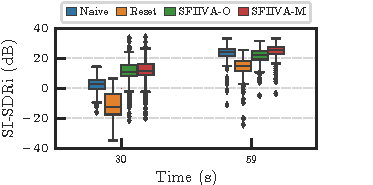
\includegraphics{figures/plots/clean/box_990.pdf}\subcaption{$\forget = 0.99 $}\label{fig:plot:box:990}
  \end{minipage}
  \caption{%
    Box-and-whisker plots of SI-SDR improvements (SI-SDRi) immediately after CMA rotation and after a sufficient time has elapsed, corresponding \SI{30}{\second} and \SI{59}{\second} in \cref{fig:plot:line}.
    The whiskers show the minima and maxima of each distribution, except for points determined to be outliers.
  }%
  \label{fig:plot:box}
\end{figure}

\subsubsection{Noisy Environments}

For a realistic simulation, we conducted experiments under the following two types of noisy environments:
\begin{description}
  \item[\texttt{babble}] Diffuse babble noise consisting of 50 speech signals.
  \item[\texttt{white}] Single interference source consisting of white noise.
\end{description}
\Cref{fig:layout:noise} shows examples of the layout of the sources and microphones in noisy environments.
Interference signals in \texttt{babble} were selected from the speech signals of the JVS dataset that were different from those used for the source signals.
The signal-to-noise ratio (SNR) is defined as
\begin{equation}
  % \text{SIR} = 10 \log _{10} \frac{\sum _{t} s _{t} ^{2}}{Q \sum _{t} n _{t} ^{2}},
  \text{SNR} = 10 \log _{10} \frac{\sum _{k=1} ^{K} \sigma _{k} ^{2}}{\sigma _{\mathrm{n}} ^{2}},
\end{equation}
where
$\sigma _{k} ^{2}$ is the variance of the $k$-th source signal at the reference microphone,
and $\sigma _{\mathrm{n}} ^{2}$ is the variance of noise signals.
After convolving room impulse responses, the variances of $k$-th source signal were scaled to $\sigma _{k} ^{2} = 1$ at the reference microphone.
Then, the variance of interferce signals was scaled so that $\text{SNR} = \SI{20}{\decibel}$.
In this experiment, we set the forgetting number $\forget$ to 0.98.
Other conditions are the same as in the noiseless case.
\begin{figure}[t]
  \centering
  \begin{minipage}[t]{.45\linewidth}
    \centering
    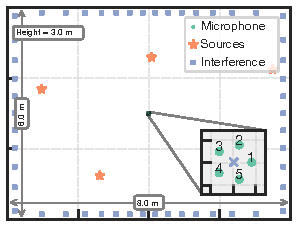
\includegraphics[width=.9\columnwidth]{figures/room_layout_noise-multi.pdf}
    \subcaption{\texttt{babble}}%
    \label{fig:layout:noise:multi}
  \end{minipage}
  \hspace{.05\linewidth}
  \begin{minipage}[t]{.45\linewidth}
    \centering
    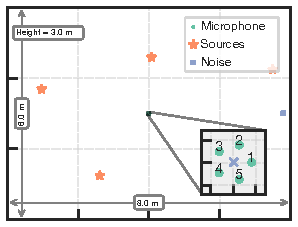
\includegraphics[width=.9\columnwidth]{figures/room_layout_noise-single.pdf}
    \subcaption{\texttt{white}}%
    \label{fig:layout:noise:single}
  \end{minipage}
  \caption{%
    Examples of room layout of noisy environments.
    The center of CMA is placed at $(\SI{4.0}{\metre}, \SI{3.0}{\metre})$ in the room with the radius of \SI{2}{\centi\metre}.
    CMA was rotated \SI{40}{\degree} counter-clockwise at \SI{30}{\second}.
    % In the zoomed plot of (b), red dots represent the microphones at the position before rotation, green dots represent the position after rotation, and the cross lines in the middle represent the center of CMA.
  }%
  \label{fig:layout:noise}
\end{figure}

\Cref{fig:plot:line:noise} shows the SI-SDRi every \SI{1}{\second} averaged over samples and channels under noisy environments.
As shown in the figure, performance between methods was consistent with the noiseless case.
Overall, the final separation performance is lower than that of the noiseless case (\cref{fig:plot:line:980}).
For \texttt{babble} and \texttt{white}, the separation performance of \texttt{white} was about \SI{10}{\decibel} lower than that of \texttt{babble}.
This is because \texttt{white} contains many components in the high frequency range that are not included in \texttt{babble} and have a negative impact on the separation performance.
\begin{figure}[t]
  \centering
  \begin{minipage}[t]{.45\textwidth}
    \centering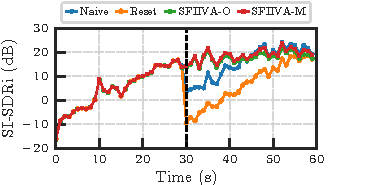
\includegraphics{figures/plots/babble-norm/line_980.pdf}\subcaption{\texttt{babble}}\label{fig:plot:line:980:babble}
  \end{minipage}
  \hspace{.05\textwidth}
  \begin{minipage}[t]{.45\textwidth}
    \centering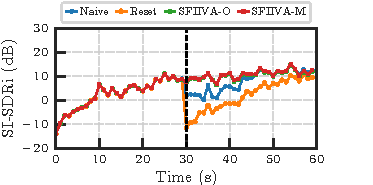
\includegraphics{figures/plots/white-norm/line_980.pdf}\subcaption{\texttt{white}}\label{fig:plot:line:980:white}
  \end{minipage}
  \caption{SI-SDR improvements (SI-SDRi) every \SI{1}{\second} with various noise.}%
  \label{fig:plot:line:noise}
\end{figure}

\subsection{Robustness against Estimation Error}

To examine the robustness against errors in measuring the angle of CMA rotation, we compared results when the measured angles used for \SFIIVAo{} and \SFIIVAm{} differed from the true angle.
As discussed in \cref{subsec:proposed:sfiivam}, we expected errors to remain when there is an error in the measured angle since \SFIIVAo{} transforms the observed signal every frame.
In contrast, \SFIIVAm{} performs the transformation only at the time of CMA rotation, so the effect of the measuring error should decrease with time.

\Cref{tab:sdr} shows the SI-SDRi (dB) averaged over samples and channels immediately after CMA rotation and after a sufficient time has elapsed with measurement errors.
The forgetting factor $\forget$ was fixed to $0.98$ in this experiment.
As expected, the SI-SDRi of both methods dropped by about \SI{8}{\decibel} \SI{30}{\second} immediately after CMA rotation,
when the measured angle was \SI{60}{\degree}, which is different from the true angle of \SI{40}{\degree}.
On the other hand, by comparing the performance at \SI{59}{\second}, which is sufficient time after CMA rotation, the performance of \SFIIVAm{} was determined to be about \SI{5}{\decibel} higher than which is that of \SFIIVAo{}.
\begin{table}[t]
  \caption{%
    Average SI-SDRi (dB) immediately after CMA rotation and after a sufficient time has elapsed.
    The length of simulated speech signals is \SI{60}{\second}, and the CMA was instantaneously rotated at \SI{30}{\second}.
    The true accurate measurement of CMA rotation was at \SI{40}{\degree} and the inaccurate measurement was at \SI{60}{\degree}.
    Forgetting factor $\forget = 0.98$.
  }%
  \label{tab:sdr}
  \centering
  \sisetup{%
    table-format=2.2,
    table-alignment-mode=format,
    table-auto-round=true,
    detect-weight=true,
  }
  \footnotesize
  \begin{minipage}[t]{.45\linewidth}
    \centering
    \subcaption{Accurate measurement.}%
    \label{tab:sdr:98}
    \begin{tabular}{lSS}
      \toprule
        Method   & \multicolumn{2}{c}{Time (s)} \\ \cmidrule{2-3}
                 &       {30} &       {59} \\
      \midrule
        SFIIVA-O &  17.988841 &  22.130434 \\ \rowcolor[gray]{0.8}
        SFIIVA-M &  18.796094 & \bfseries  25.623199 \\
      \bottomrule
    \end{tabular}
  \end{minipage}
  \hspace{.05\linewidth}
  \begin{minipage}[t]{.45\linewidth}
    \centering
    \subcaption{Inaccurate measurement.}%
    \label{tab:sdr:98}
    \begin{tabular}{lSS}
      \toprule
        Method   & \multicolumn{2}{c}{Time (s)} \\ \cmidrule{2-3}
                 &       {30} &       {59} \\
      \midrule
        SFIIVA-O &   9.922167 &  20.262950 \\ \rowcolor[gray]{0.8}
        SFIIVA-M &   9.980653 &  \bfseries 25.626287 \\
      \bottomrule
    \end{tabular}
  \end{minipage}
\end{table}

\subsection{Difference in Beam Pattern}

In this subsection, we selected one example to focus on the difference between the two proposed methods \SFIIVAo{} and \SFIIVAm{}.
\Cref{fig:plot:beam} shows the beam patterns of the demixing matrices calculated by each method.
\Cref{fig:plot:bp:ref} is the result calculated before the rotation.
\Cref{fig:plot:bp:sfiivao,fig:plot:bp:sfiivam} are the results with the demixing matrices calculated using \SFIIVAo{} and \SFIIVAm{}, respectively, after the rotation.
Dark regions in each plot represent nulls in a certain direction.
In the case of online AuxIVA, the desired result is that the direction of the estimated source is toward the brighter regions, and that of the others is toward the darker region.
As shown in \cref{fig:plot:beam,fig:plot:bp:ref}, the results were similar to each other, and only the results in \cref{fig:plot:bp:sfiivam} were different from the each other.
The dark regions in \cref{fig:plot:bp:ref,fig:plot:bp:sfiivao} were nearly in the desired directions since \SFIIVAo{} approximately canceled the rotation of the CMA and thus updated the demixing matrices in the same direction even after the rotation.
For \SFIIVAm{}, the bright areas should be in the direction viewed from the position after the rotation, \emph{i.e.}, \SI{40}{\degree} less anti-clockwise than the previous result in this case.
The nulls may not be precisely formed in some frequency bands where the source signal is inherently weak because it does not affect the separated signal very much.
Looking at the high-frequency bands of each beam pattern, there are several cases where bright regions are visible outside of the target signal, such as Est. 4 in \cref{fig:plot:bp:sfiivam}.
We suppose this result might happen since the 4th estimated signal in high-frequency bands was accidentally weak.
\begin{figure}[t]
  \centering
  \begin{minipage}[t]{\linewidth}
    \centering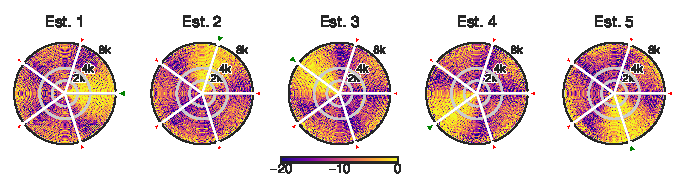
\includegraphics{figures/plots/beam-pattern/ref.pdf}\subcaption{Before rotation.}\label{fig:plot:bp:ref}
  \end{minipage}
  \begin{minipage}[t]{\linewidth}
    \centering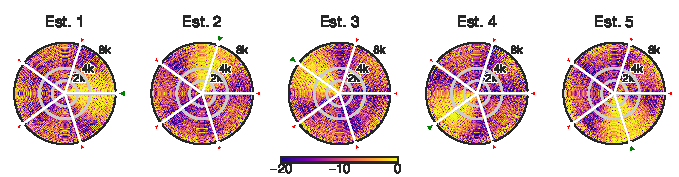
\includegraphics{figures/plots/beam-pattern/rot_sfiiva-o.pdf}\subcaption{\SFIIVAo{} after rotation.}\label{fig:plot:bp:sfiivao}
  \end{minipage}
  \begin{minipage}[t]{\linewidth}
    \centering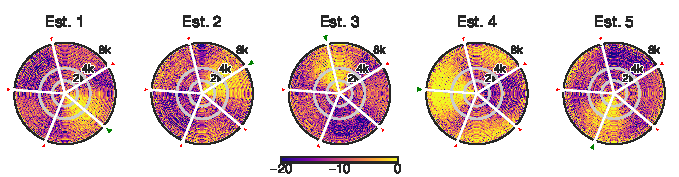
\includegraphics{figures/plots/beam-pattern/rot_sfiiva-m.pdf}\subcaption{\SFIIVAm{} after rotation.}\label{fig:plot:bp:sfiivam}
  \end{minipage}
  \caption{%
    Beam patterns of demixing matrices.
    The five plots are the beam patterns of the frequency-wise demixing matrices calculated by each method.
    The radial direction of each plot represents the frequency, and the tangential direction represents the angle from the center of the CMA.
    The light and dark colors represent the gain in decibels.
    The five triangles in each plot indicate the true direction of the source, with green representing the target source and red the interference source.
  }%
  \label{fig:plot:beam}
\end{figure}

\section{Conclusion}\label{sec:conclusion}

In this study, sound field interpolation (SFI) for an equally spaced circular microphone array (CMA) was applied to online auxiliary-function-based independent vector analysis (OIVA).
We have proposed the following two new methods: a simple combination of SFI and OIVA, and a practical method based on parameter transformations.
Simulation experiments have confirmed that SFI improved the robustness of OIVA against CMA rotation.
Future work includes combining this method with self-rotation angle estimation such as \cite{Lian:2021:APSIPA}, under-determined BSS methods such as \cite{Yamaoka:2019:EUSIPCO,Yamaoka:2021:ASLP}, over-determined BSS methods such as \cite{Scheibler:2019:WASPAA,Ikeshita:2020:ICASSP}, and extending it to real-time processing.

\section*{Biographies}

\noindent\normalsize\textbf{Taishi Nakashima}
received his B.E. in Engineering from Osaka University, Osaka, Japan, in 2019 and his M.S. in Informatics from Tokyo Metropolitan University, Tokyo, Japan, in 2021.
He is pursuing a Ph.D. at Tokyo Metropolitan University and has received the JSPS Research Fellowship (DC1) in April 2021.
He is an esteemed Student Member of the Acoustical Society of Japan (ASJ) and the IEEE Signal Processing Society (SPS).
He received the 24th Best Student Presentation Award of ASJ, the 16th IEEE SPS Japan Student Conference Paper Award in 2022, and the Top 3\% Recognition at ICASSP 2023.
His research interests primarily focus on blind source separation and acoustic signal processing.
\\

\noindent\normalsize\textbf{Yukoh Wakabayashi}
received the his B.E. and M.E. degrees from Osaka University, Osaka, Japan, in 2008 and 2010, respectively, and his Ph.D. degree from Ritsumeikan University, Shiga, Japan, in 2017.
He joined Rohm, Inc., Kyoto, Japan, in 2010, and was an assistant researcher at Kyoto University from 2012 to 2014.
He was a recipient of the JSPS Research Fellowship for Young Scientists DC2 from 2016 to 2017.
He was an affiliate assistant professor with Ritsumeikan University from 2018 to 2020.
He is currently an assistant professor at the Department of Computer Science and Engineering, Toyohashi University of Technology, Aichi, Japan, and the Faculty of Systems Design, Tokyo Metropolitan University, Tokyo, Japan.
His research interests include acoustic signal processing, speech phase processing, array signal processing, and speaker diarization.
He is a member of the Institute of Electrical and Electronics Engineers, the Institute of Electronics, Information and Communication Engineers, and Acoustical Society of Japan.
\\

\noindent\normalsize\textbf{Nobutaka Ono}
received his B.E., M.S., and Ph.D. degrees from The University of Tokyo, Japan, in 1996, 1998, and 2001, respectively.
He became a research associate in 2001 and a lecturer in 2005 at The University of Tokyo.
He moved to the National Institute of Informatics in 2011 as an associate professor and then to Tokyo Metropolitan University in 2017 as a full professor.
His research interests include acoustic signal processing, especially microphone array processing, source localization and separation, machine learning, and optimization algorithms.
He is a member of IEEE, EURASIP, APSIPA, IPSJ, IEICE, and ASJ.
He was a member of the IEEE Audio and Acoustic Signal Processing (AASP) Technical Committee from 2014 to 2019.
He served as Associate Editor of IEEE Transactions on Audio, Speech, and Language Processing from 2012 to 2015.
He received the best paper award at APSIPA ASC in 2018 and 2021 and Sadaoki Furui Prize Paper Award from APSIPA in 2021.

\printbibliography

\end{document}
